\newpage
\section{Durchführung}
\label{sec:Durchfuehrung} %darauf wird verlinkt in Vorbereitungsteil Elastisches Nachwirken!
\subsection{Versuchsaufbau}

\begin{figure}[h]
    \begin{subfigure}[c]{0.5\textwidth}
        \centering
        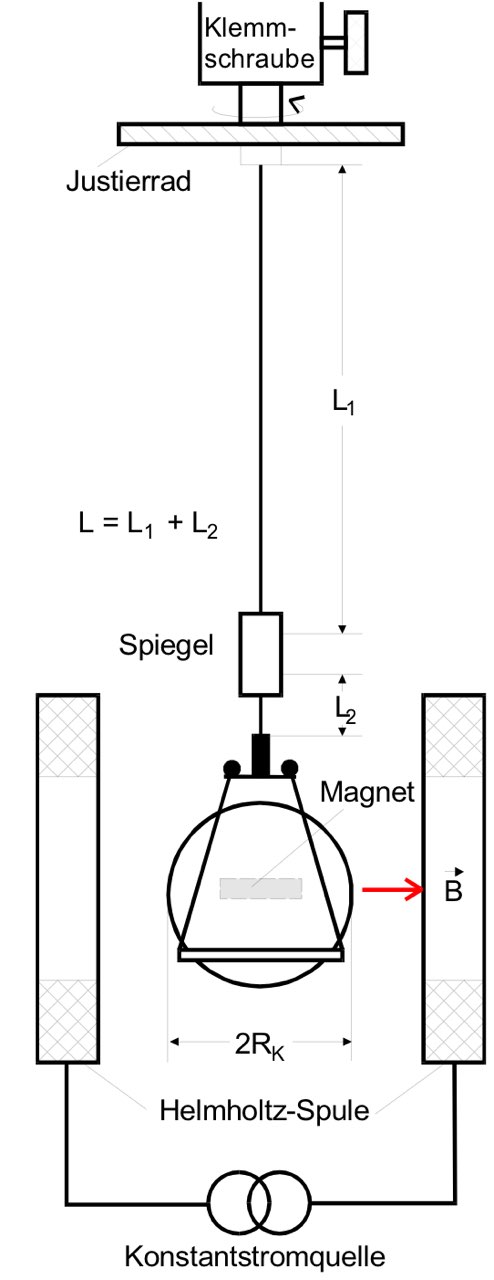
\includegraphics[width=0.3\textwidth, height=0.7\textwidth]{bilder/magnet_apperatur.jpeg}
        \subcaption{Versuchsaufbau Skizze,\cite[9]{Anleitung}}        
        \label{fig:Torsion_apperatur}
    \end{subfigure}
    \begin{subfigure}[c]{0.5\textwidth}
        \centering
        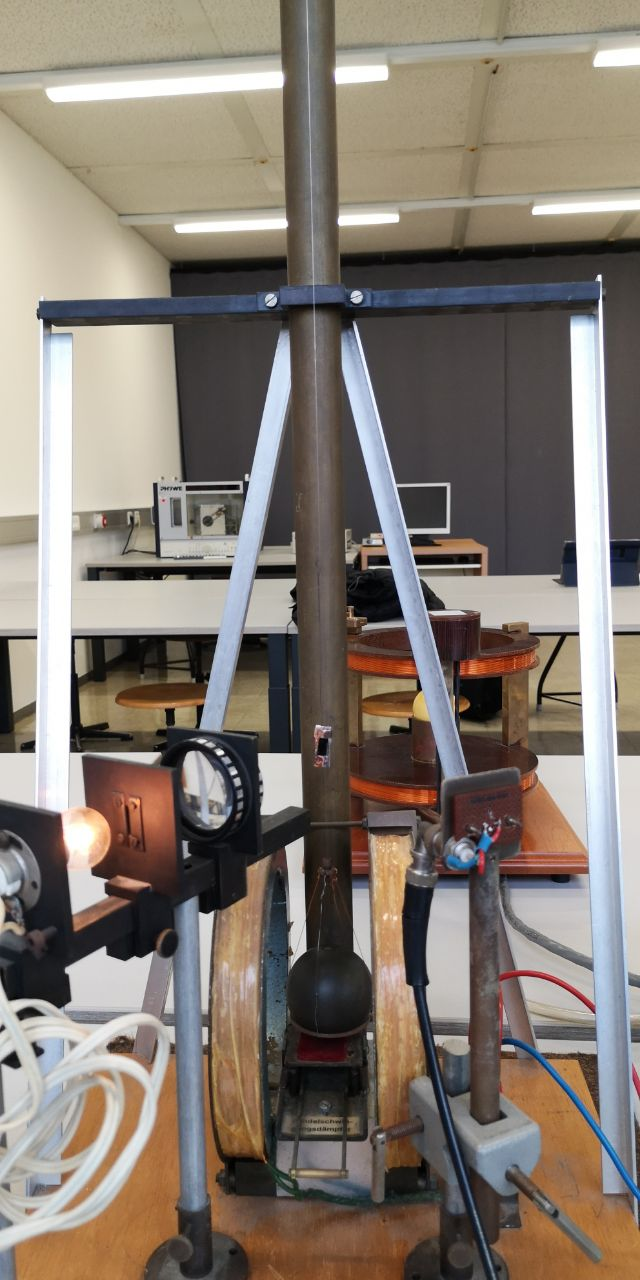
\includegraphics[width=0.3\textwidth, height=0.7\textwidth]{bilder/Foto_Versuchsaufbau.jpeg}
        \subcaption{Foto des Versuchsaufbaus}
        \label{fig:Foto_Versuchsaufbau}
    \end{subfigure}
\end{figure}

Die Kugel soll im Versuch nicht pendeln um Fehler in den Versuchswerten zu vermeiden.
Daher ist unter der Kugel eine Vorrichtung angebracht um nach jeder Messreihe die Pendelbewegung zu dämpfen.\\

Um die Periodendauer zu messen muss mithilfe des Rings an der Aufhängung des Drahtes der Draht verdreht werde,
wobei darauf geachtet werden muss dass der Spiegel bei der Schwingung den Lichtstrahl über die Photodiode lenkt.\\

Das Experiment zur Bestimmung des Elastizitätsmoduls aus der Schallgeschwindigkeit war nicht durchführbar,
daher haben wir hierfür einen vorgegebenen Wert.\\

-Kugel darf nicht wobbeln/pendeln\\
-Torsion muss über lichtschranke erfolgen\\
-Messung der Schallgeschwindigkeit entfällt\\

\subsection{Die Periodendauer T}
Im ersten Versuch darf an der Helmholtzspule kein strom anliegen da ausschließlich die Elastizität des Stoffes einfluss auf die Periodendauer haben soll.
Zu Beginn des versuchs wird der Magnet im inneren der Kugel parallel zum Draht eingestellt.
Die Lampe am Versuchsaufbau wird eingeschaltet und das Licht trifft über eine Linse auf den am Draht befestigten Spiegel.
Wenn der Draht nun ausgelenkt wird, wird läuft der Lichtstrahl durch den mitschwingenden Spiegel periodisch über die Photodiode.\\
Die Photodiode ist über eine elektrische schaltung an die Quarzuhr gekoppelt.
Die elektrische Schaltung lässt über eine bistabile Kippstufe (Flip-Flop) das erste Signal passieren um die Stoppuhr zu starten.
Mithilfe der bistabilen Kippstufe wird das 2. Signal unterdrückt.
Das dritte Signal stoppt die Quarzuhr und durch die monostabile Kippstufe und einem weiteren Flip-Flop wird die Uhr mit dem 4. Signal zurück gesetzt.\\

\subsection{Die Periodendauer T im B-Feld}
Um die Stärke des Permanentmagneten in der Kugel zu berechnen muss dieser senkrecht zum draht ausgerichtet werden, da so die Fehler durch das Erdmagnetfeld minimiert werden.
Die Stromstärke an der Helmholtzspule wird nun von 0.1 Ampere bis 1 Ampere in 0.1 Ampere Schritten erhöht und für jede Stromstakre werden 10 Wertte gemessen.